\documentclass[a4paper]{report}

%====================== PACKAGES ======================
\usepackage{hyperref}
\usepackage[french]{babel}
\usepackage[utf8x]{inputenc}
%pour gérer les positionnement d'images
\usepackage{float}
\usepackage{amsmath}
\usepackage{graphicx}
\usepackage[colorinlistoftodos]{todonotes}
\usepackage{url}
%pour les informations sur un document compilé en PDF et les liens externes / internes
\usepackage{hyperref}
%pour la mise en page des tableaux
\usepackage{array}
\usepackage{tabularx}
%pour utiliser \floatbarrier
%\usepackage{placeins}
%\usepackage{floatrow}
%espacement entre les lignes
\usepackage{setspace}
%modifier la mise en page de l'abstract
\usepackage{abstract}
%police et mise en page (marges) du document
\usepackage[T1]{fontenc}
\usepackage[top=2cm, bottom=2cm, left=2cm, right=2cm]{geometry}
%Pour les galerie d'images
\usepackage{subfig}

\begin{document}

%--------------------------------------------------_Debut Page Titre

\begin{titlepage}
\begin{center}

% Upper part of the page. The '~' is needed because only works if a paragraph has started.

\includegraphics[width=0.35\textwidth]{./logo}~\\[1.5cm]



\textsc{\LARGE Université de La Reunion}\\[0.2cm]
\text{Brice VIRASSAMY 36004977}


\textsc{\Large }\\[0.5cm]




% Title

\huge \bfseries File d'entier\\



\end{center}

% Fin de page
\vfill

\large {Session 2018/2019}

\end{titlepage}

%-----------------------------------------------_Fin de Page Titre

\newpage
-
%ne pas numéroter cette page
\thispagestyle{empty}
\newpage

%------------------------------------------------_Résumé

\begin{abstract}
    
    \begin{spacing}{1.5}
    En résumé, cet exercice du TP consiste à modéliser un producteur et des consommateurs (d'un domaine quelconque) avec un système de file d'attente. Le producteur fournit à la file d'attente jusqu'à ce qu'elle soit pleine et les consommateurs consomment jusqu'à l'indisponibilité de la ressource, autrement dit lorsqu'il n'y a plus de produit dans la file d'attente. j'ai choisi de rajouter la possibilité de mettre en pause les consommateurs et le producteur pour que même s'il y ait disponibilité de ressources ou même si la file n'est pas pleine, le producteur et les consommateurs arrêtent leurs activités. Une interface graphique a aussi été rajouter pour l'utilisateur du programme (interface en java et python). 
    \end{spacing}
    
\end{abstract}


%------------------------------------------------_Fin Résumé

%------------------------------------------------_Table des matieres

\tableofcontents
\thispagestyle{empty}
\setcounter{page}{0}

\newpage
\renewcommand{\arraystretch}{1.5}

%------------------------------------------------_Fin Tb des matieres

~
\thispagestyle{empty}
%recommencer la numérotation des pages à "1"
\setcounter{page}{0}
\newpage


%-----------------------------____Début rédaction

\chapter{Introduction}

\section{Objectifs}

Les objectifs à réaliser sont les suivants :

\begin{itemize} 
\item Faire en sorte que le producteur/consommateur ne puisse pas produire/consommer quand la file est pleine/vide.
\item Rajouter la fonctionnalité de pause qui a été énoncer.
\item Proposer une interface graphique cohérente avec le sujet.
\end{itemize}

\section{Plan}

\begin{itemize}
\item Dans un 1er temps : Nous parlerons des recherches et apprentissages préliminaires à la rédaction du code
\item Dans un 2nd temps : Nous traiterons les points importants communs aux deux langages.
\item Dans un 3eme temps : Nous examinerons l'interface graphique en java.
\item Dans un 4eme temps : Nous examinerons l'interface graphique en python.
\end{itemize}
    


%___________


\chapter{Les préliminaires}

\section{En Java}

En amont du programme java, je me suis donc renseigné sur comment modéliser l'idée que j'avais concernant l'interface graphique. J'avais des connaissances, solides sur certains points où je savais exactement quel code effectuer mais sur d'autres points notamment le traitement des "JLabels" après leurs créations, j'avais des lacunes donc j'ai consulté différents sites qui traités points par points des éléments possibles d'une interface graphique, mais je ne savais pas comment assembler tout cela donc j'ai décidé de reprendre depuis le début l'apprentissage de l'interface graphique java à travers le cours de java sur le site openclassroom.

\section{En Python}

En amont du programme python, comme pour le programme en python je me suis renseigneé sur comment modéliser l'idée que j'avais. Le problème était que je n'ai jamais programmé d'interface graphique en python, c'était donc une découverte pour moi. Le prof nous a indiqué quel était le nom de l'interface graphique (TKinter) et un cours sur le site openclassroom pour nous permettre de manière autonome de s'approprier cette librairie. Je suis donc parti de zéro par rapport à java concernant l'interface graphique et j'ai suivi rigoureusement le cours, mais en conséquent j'ai pris plus de temps sur la programmation en python par rapport à ce point.


%_____________

\chapter{Points importants}

\section{Le test primordial}
\paragraph{
En lien avec les objectifs, les producteurs et les consommateurs ne doivent pas manipuler la file si elle est vide pour le consommateur ou si elle est pleine pour le producteur. Ceci a été réaliser grâce aux codes suivants :}

\textsc{En java, dans la file, dans les méthodes enfiler et defiler un element) :}
\begin{verbatim}
while(tabFile.size()==MAX) wait();
tabFile.add(e);
notifyAll();
\end{verbatim}

\begin{verbatim}
while(tabFile.size()==0) wait();
int e = tabFile.get(0);
tabFile.remove(0);
notifyAll();
\end{verbatim}


\textsc{En Python, dans la file, dans les méthodes enfiler et defiler un element) :}

\begin{verbatim}
with self.cond:
    while(len(self.tabFile)==20):
        self.cond.wait()
    self.tabFile.append(e)
    self.cond.notifyAll()    
\end{verbatim}

\begin{verbatim}
with self.cond:
    while(len(self.tabFile)==0):
          self.cond.wait()
    e = self.tabFile[0]
    del self.tabFile[0]
    self.cond.notifyAll()
\end{verbatim}

Ces codes testent si la file est vide ou si elle est pleine. Si elle est pleine le producteur ne peut plus rajouter. Si elle est vide le consommateur ne peut plus consommer.

\section{La mise en pause}

\paragraph{Toujours en accord avec les objectifs, la mise en pause doit pouvoir s'effectuer correctement, la file ne doit pas se remettre dans son état initial à la mise en pause des threads, c'est à dire avec zéro élément (sauf si tout a été consommer au préalable). je vais expliquer concrètement comment cela fonctionne.
Au lancement du programme je lance une méthode, startThread() qui lance les threads qui ont été crée:}

\textsc{En java :}
\begin{verbatim}
	public void startThread() {
		createThread();
		prod.start();
		for(int i = 0; i<consos.length;i++) { consos[i].start(); }
	}
\end{verbatim}
\textsc{En python :}
\begin{verbatim}
def startThread(self):
    self.createThread()
    self.prod.start()
    for threadConso in self.consos:
        threadConso.start()
\end{verbatim}
%_____________
\paragraph{Ensuite si je clique sur stop, la méthode stopThread() est lancée et stop les threads, mais on ne veut pas stopper, on veut mettre en pause.
Ce qu'il faut savoir, c'est que les éléments des Threads initiaux sont stockés en attribut de la classe fenêtre donc jamais effacé, quand je reclique sur startThread() cela recrée des nouveaux Threads mais avec les éléments des Threads initiaux donc cela permet de reprendre avec les "mêmes threads". Le bouton start/stop simule donc bien une pause. Voilà la méthode stopThread():}

\textsc{En java :}
\begin{verbatim}
public void stopThread(){
prod.interrupt();
for(int i = 0; i<consos.length;i++) { consos[i].interrupt(); }
labProd.setText("");
labConso.setText("");
repaint();
}
\end{verbatim}
\textsc{En python :}
\begin{verbatim}
def stopThread(self):
    self.prod.interrupt()
    for threadConso in self.consos:
        threadConso.interrupt()
    self.labConso.config(text="")
    self.labProd.config(text="")
        
    self.labFile.update()
    self.labConso.update()
    self.labProd.update()
\end{verbatim}
%_____________

\chapter{Architecture de l'interface graphique en Java}

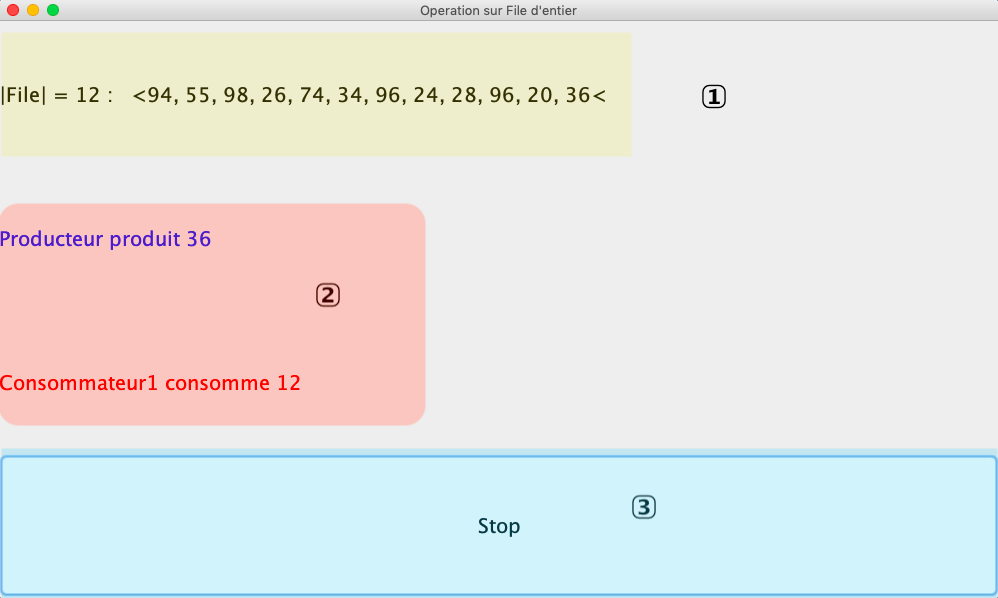
\includegraphics[width=1\textwidth]{./fen_java.png}

\paragraph{
L'interface graphique est une fenêtre JFrame.
En 1, nous avons la file. En 2, les threads producteurs et consommateurs.
En 3, le bouton start/stop pour mettre en pause ou relancer les threads.
En 1 et 2 tout a été constitué avec des JLabels. En 3, c'est un bouton et il a été constitué avec un JButton.}

\paragraph{Code de création des éléments :}

\begin{verbatim}
this.labFile = new JLabel();
		labFile.setText("< <");
		labFile.setForeground(Color.BLACK);
		labFile.setFont(new Font("Courrier New", Font.PLAIN, 20));
		
		this.labProd = new JLabel();
		labProd.setForeground(Color.BLUE);
		labProd.setFont(new Font("Courrier New", Font.PLAIN, 20));
		
		this.labConso = new JLabel();
		labConso.setForeground(Color.RED);
		labConso.setFont(new Font("Courrier New", Font.PLAIN, 20));
		
		JButton stopAndStart = new JButton("Start");
		stopAndStart.setFont(new Font("Courrier New", Font.PLAIN, 20));
\end{verbatim}

\paragraph{La methode setText() permet d'éditer le texte présent dans le Jlabel, setForeground() permet d'éditer la couleur et setFont() la couleur}


%_____________

\chapter{Architecture de l'interface graphique en Python}

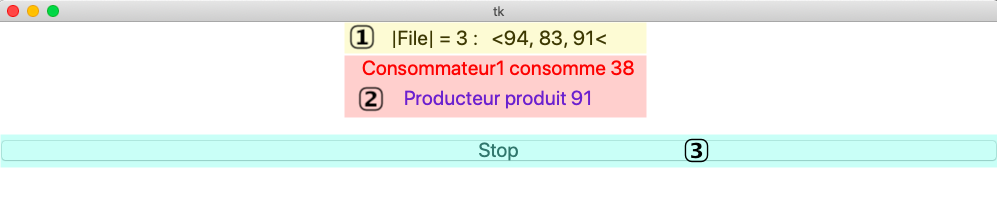
\includegraphics[width=1\textwidth]{./fen_pyt.png}

\paragraph{
L'interface graphique est une fenêtre Frame. Comme pour Java, en 1 nous avons la file, en 2 les threads et en 3 le bouton start/stop. En 1 et 2 tout a été constitué en Label (python) et 3 avec un Button (python)}

\paragraph{Code de création des éléments :}

\begin{verbatim}
    self.labFile = Label(self,text="<  <",font=("Courrier New",20))
    self.labProd = Label(self,text="", fg="blue",font=("Courrier New",20))
    self.labConso = Label(self,text="", fg="red",font=("Courrier New",20))
    self.stopAndStart = Button(self, text="Start", command =self.cliquer,font=("Courrier New",20))
    self.stopAndStart.pack(side="bottom", fill=BOTH)
    self.labProd.pack(side="bottom",fill=BOTH)
    self.labConso.pack(side="bottom",fill=BOTH)
    self.labFile.pack(side="bottom",fill=BOTH)
\end{verbatim}

\paragraph{Les attributs text, fg (foreground en java), font sont équivalents aux méthodes avec le même nom en java. L'attribut command attend une fonction comme valeur, cette fonction sera exécutée au clic sur le bouton. La méthode pack() avec les attributs side et fill sert au positionnement dans la fenêtre Frame}

%______________

\chapter{Conclusion}

\paragraph{Pour conclure, les objectifs énoncés ont tous été réaliser, la production et la consommation respectent ce qui a été imposer. La mise en pause est fonctionnelle. L'interface graphique est présente et cohérente avec le sujet. Pour améliorer le programme on pourrait améliorer l'interface graphique, principalement en python. On pourrait aussi rajouter une fonctionnalité pour saisir les threads directement dans l'interface graphique. }

%_______________

\chapter{Bibliographie}

\begin{itemize}
    \item Cours Interface Graphique Java :
    \url{https://openclassrooms.com/courses/apprenez-a-programmer-en-java/le-fil-rouge-une-animation}
    \item Cours Interface Graphique Python : 
    \url{https://openclassrooms.com/fr/courses/235344-apprenez-a-programmer-en-python/234859-des-interfaces-graphiques-avec-tkinter}
    
\end{itemize}


%-----------------------------____Fin rédaction



\end{document}

